\chapter{Plataforma de desarrollo}
\label{cap:capitulo3}

\begin{flushright}
\begin{minipage}[]{10cm}
\emph{Quizás algún fragmento de libro inspirador...}\\
\end{minipage}\\

Autor, \textit{Título}\\
\end{flushright}

\vspace{1cm}

Escribe aquí un párrafo explicando brevemente lo que vas a contar en este capítulo. En este capítulo, explica qué has usado a nivel hardware y software para poder desarrollar tu trabajo: librerías, sistemas operativos, plataformas, entornos de desarrollo, etc.

\section{Raspberry Pi 4 Model B}
\label{sec:rpi}

La Raspberry Pi 4 Model B (Figura \ref{fig:raspberry2}) es la plataforma hardware de bajo coste escogida para este proyecto. Debido a la gran comunidad de desarrolladores y usuarios que posee, además de las especificaciones ofrecidas (Cuadro \ref{cuadro:especificaciones_rpi4}) por su escaso precio (65,44 \euro\footnote{Distribuidor oficial de Raspberry: \url{https://www.kubii.es/40-raspberry-pi-3-2-b}}), es la plataforma más usada por la mayoría del público.\\

\begin{figure} [h!]
  \begin{center}
    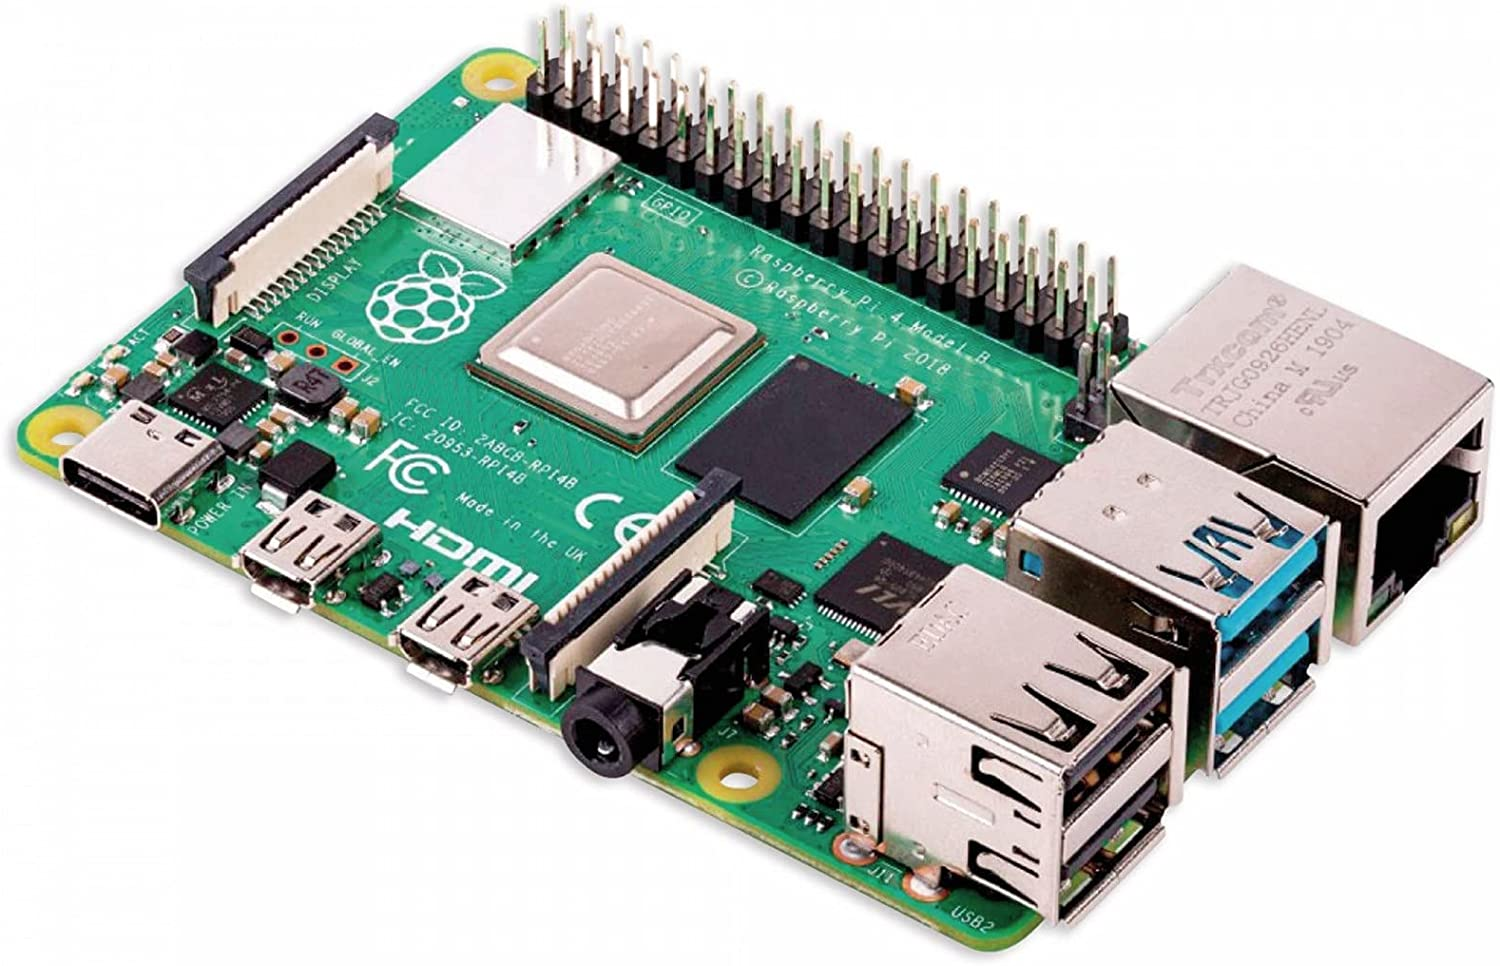
\includegraphics[width=9cm]{figs/raspberry.jpg}
  \end{center}
  \caption{Raspberry Pi 4b.}
  \label{fig:raspberry2}
\end{figure}

Sus características más atractivas ---entre otras--- son su bajo consumo energético, su pequeño tamaño y por lo tanto mínimo peso, su alta conectividad y puertos (red WIFI, Bluetooth, Ethernet, USB2 y USB3, HDMI, etc.) y la gran fluidez que posee su sistema operativo (Sección \ref{sec:raspberry_pi_os}). Todo esto la convierte en una auténtica joya y son cada vez más usuarios los que la utilizan en diversos proyectos. Podemos encontrarla ---por ejemplo--- como centro doméstico inteligente para controlar la domótica de una casa o incluso en sectores más profesionales formando parte de la arquitectura de algunos robots. Esto último es lo más interesante, para nosotros, dentro de los múltiples usos que tiene una Raspberry.\\

\begin{table}[H]
\begin{center}
\begin{tabular}{|>{\arraybackslash}m{3cm} | >{\arraybackslash}m{6cm} |}
     \hline
     Procesador & Broadcom BCM2711 (4 núcleos Cortex-A72 (ARM v8), 64-bit, 1.5Ghz) \\ \hline
     Tarjeta gráfica & Broadcom VideoCore VI (integrada en el procesador) \\ \hline
     Memoria RAM & 4 GB LPDDR4-3200 SDRAM \\ \hline
     \multirow{3}{*}{Conexión}& WIFI 2.4 GHz y 5 GHz\\
     & Bluetooth 5.0/BLE\\
     & Gigabit Ethernet \\ \hline
     \multirow{5}{*}{Puertos}& 2 x micro-HDMI (4K 60 Hz)\\
     & MIPI Display Serial Interface \\
     & MIPI Camera Serial Interface \\
     & Jack Audio/Vídeo \\
     & Slot para micro-SD \\ \hline
     \multirow{2}{*}{Alimentación} & 5V por USB-C (3A mínimo) \\
     & 5V por GPIO (3A mínimo) \\ 
     \hline
 \end{tabular}
\caption{Especificaciones técnicas de la Raspberry Pi 4 Model B.}
\label{cuadro:especificaciones_rpi4}
\end{center}
\end{table}

Muchos de los robots son de tamaño reducido y no tienen el espacio suficiente como para acoplar una gran estación de procesamiento, por lo tanto en esos casos es muy común usar algún modelo de Raspberry como unidad central. Incluso en robots grandes se suelen utilizar también para realizar el control de zonas concretas, por ejemplo de los ojos de un humanoide. Por lo tanto, nuestro sistema de detección de emociones corriendo en la Raspberry Pi 4 Model B puede servir de gran ayuda a la hora de construir uno de estos robots comentados anteriormente que sólo tienen la capacidad de albergar una placa de tamaño reducido, o que simplemente los desarrolladores de dicho robot quieren ahorrar dinero en costes.

\subsection{Raspberry Pi OS}
\label{sec:raspberry_pi_os}

Raspberry Pi OS (Figura \ref{fig:captura_rpios}) es el sistema operativo oficial para Raspberry. Es un sistema operativo gratuito basado en Debian optimizado específicamente para el hardware de la Raspberry Pi, por lo tanto es el que mayor rendimiento nos ofrecerá frente a otros como Ubuntu (que también puede ser instalado). Además, está en constante desarrollo y continuamente se está mejorando su estabilidad y funcionalidad. Es por todo ello que será el sistema operativo elegido en nuestro proyecto, sobre todo por su alto rendimiento (algo esencial para impulsar el desempeño de nuestro sistema de detección de emociones).\\

\begin{figure} [h!]
  \begin{center}
    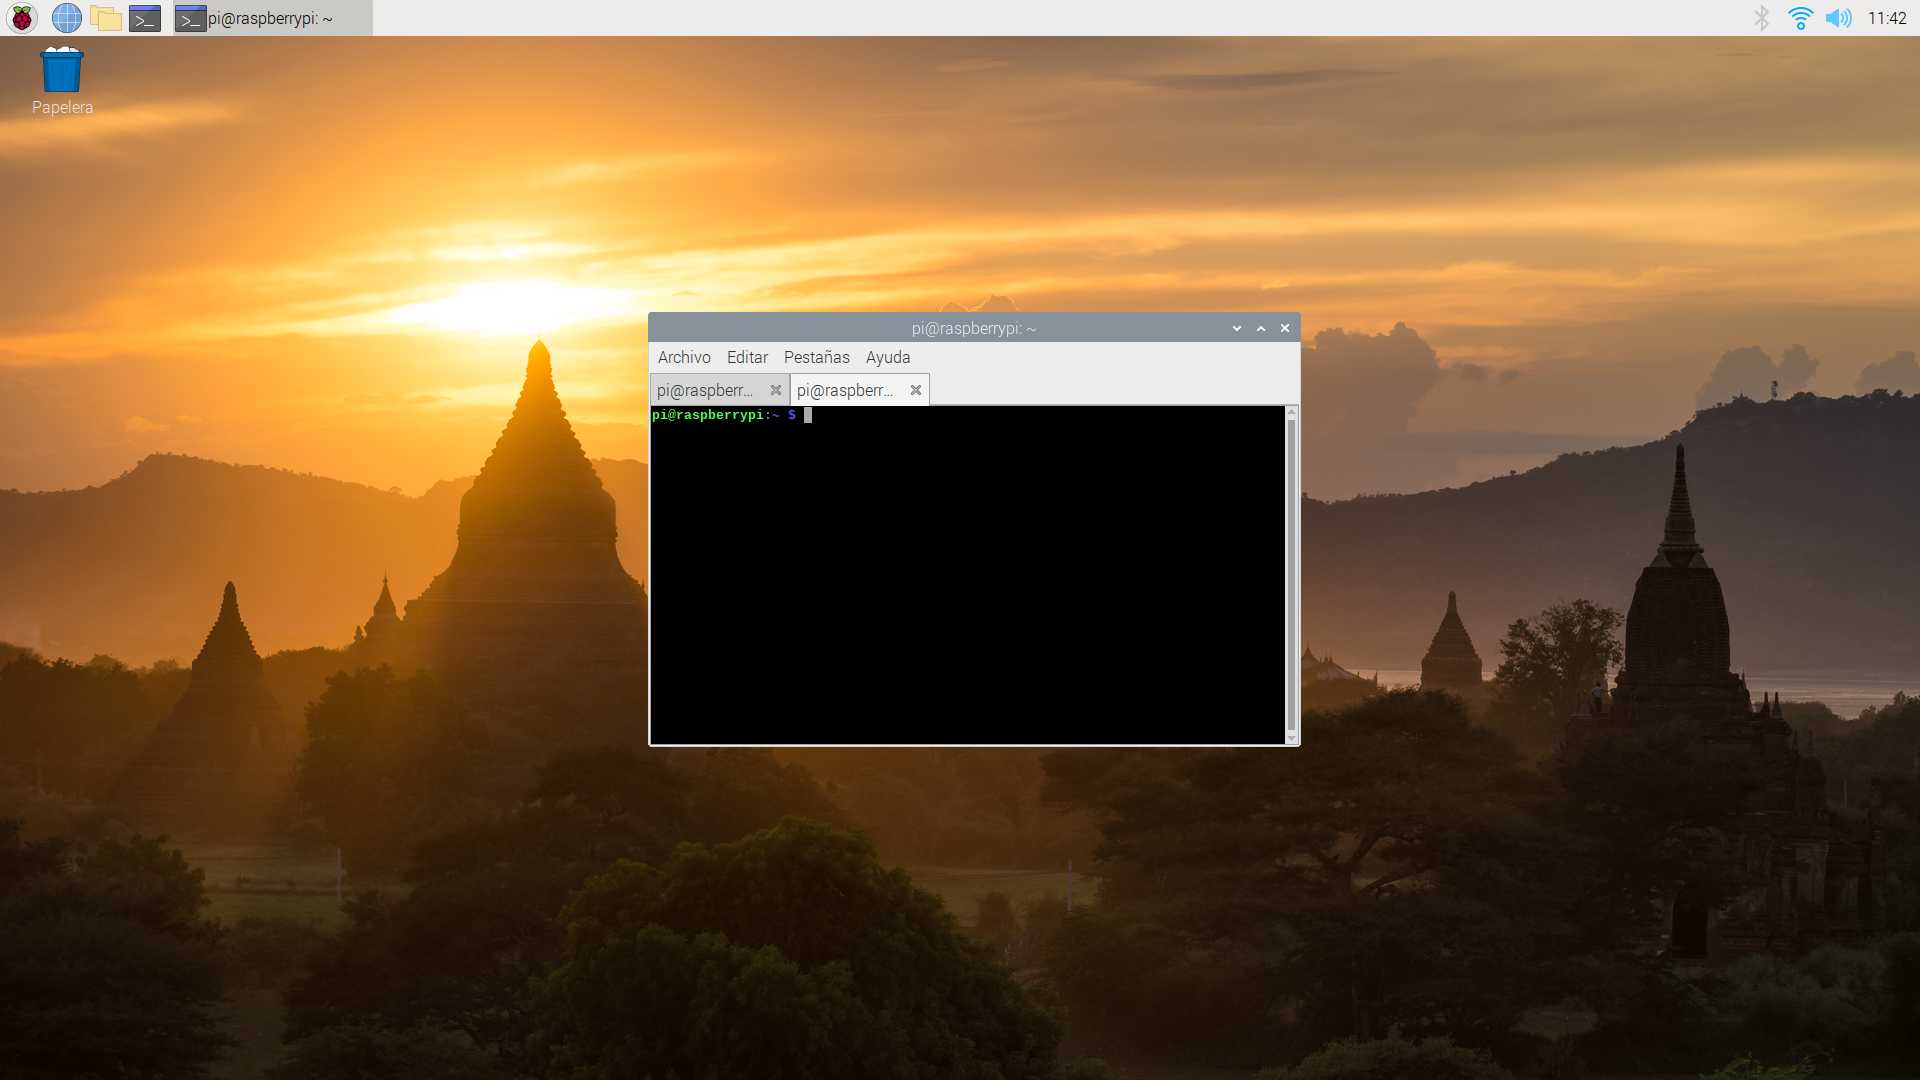
\includegraphics[width=13cm]{figs/captura_rpios.png}
  \end{center}
  \caption{Captura de pantalla de Raspberry Pi OS.}
  \label{fig:captura_rpios}
\end{figure}

La versión de Raspberry Pi OS escogida ha sido Raspberry Pi OS Legacy (Cuadro \ref{cuadro:especificaciones_rpios}). Se ha elegido dicha versión porque, de todas las disponibles, ha sido la única en la que se ha conseguido instalar una versión de ROS/ROS2 (en concreto, ROS Noetic). Además, aunque las versiones de Raspberry Pi OS de 64-bit ofrecían más rendimiento, todavía no estaban maduras y no ofrecían total compatibilidad con todas las librerías usadas en el presente trabajo.

\begin{table}[H]
\begin{center}
\begin{tabular}{|>{\arraybackslash}m{4cm} | >{\arraybackslash}m{4cm} |}
     \hline
     Fecha de lanzamiento & 4 de Abril de 2022 \\ \hline
     Sistema & 32-bit \\ \hline
     Versión del Kernel & 5.10 \\ \hline
     Versión de Debian & 10 (buster) \\ \hline
 \end{tabular}
\caption{Especificaciones de Raspberry Pi OS Legacy.}
\label{cuadro:especificaciones_rpios}
\end{center}
\end{table}

\subsection{Raspberry Pi Camera Module V2.1}
\label{sec:rpi_camera}

La Raspberry Pi Camera es la cámara oficial desarrollada por Raspberry para ser utilizada en sus placas. Para este trabajo, se ha hecho uso de la versión 2.1 (Cuadro \ref{cuadro:especificaciones_rpi_camera}). Es una cámara de alta definición (3280x2464) que se conecta a cualquier Raspberry Pi compatible a través de una interfaz de bus CSI-2. Además de vídeo de alta calidad, ofrece una reducción de la contaminación de la imagen (ruido o manchas).\\

\begin{table}[H]
\begin{center}
\begin{tabular}{|>{\arraybackslash}m{4cm} | >{\arraybackslash}m{6cm} |}
     \hline
     Sensor de imagen & Sony IMX 219 PQ CMOS \\ \hline
     Resolución de imagen & 3280x2464 (8-megapixeles) \\ \hline
     \multirow{2}{*}{Resolución de vídeo}& 1080p 30fps\\
     & 720p 60fps \\ \hline
     Conexión & Cable plano de 15 pines, MIPI Camera Serial Interfaze (CSI-2)\\ \hline
     Peso & 3g \\ \hline
     Dimensiones & 23.86 x 25 x 9 mm \\ \hline 
 \end{tabular}
\caption{Especificaciones de Raspberry Pi Camera Module V2.1.}
\label{cuadro:especificaciones_rpi_camera}
\end{center}
\end{table}

Se ha decidido escoger la Raspberry Pi Camera Module V2.1 en vez de una versión convencional de WebCam (USB) debido a las siguientes ventajas:

\begin{itemize}
    \item \textit{Mayor framerate.} Gracias a que la Raspberry Pi 4 Model B tiene un puerto dedicado para conectar la Raspberry Pi Camera, es posible conseguir una gran velocidad de fotogramas. Esto es debido a que esa conexión especial permite que la codificación vaya dirigida directamente a la GPU y sólo haya un pequeño impacto en la CPU, dejándola libre para otros usos. En cambio, una WebCam conectada por USB utiliza directamente la CPU, y mover datos a través de un USB es bastante costoso para un sistema de recursos limitados.
    
    \item \textit{Mayor calidad de imagen.} Es cierto que también existen WebCam con una calidad de imagen muy buena, pero su precio es elevado. Por lo tanto, la Raspberry Pi Camera acaba ganando en cuanto a calidad de imagen si realizamos la comparativa en el mismo rango de precio (29,14 \euro\footnote{Distribuidor oficial de Raspberry: \url{https://www.kubii.es/318-camaras-sensores}}). Sin embargo, este no es un apartado muy relevante porque finalmente en el sistema de detección de emociones no hacemos uso de la máxima resolución para aumentar el rendimiento.
    
    \item \textit{Menor tamaño.} El tamaño tan compacto de la Raspberry Pi Camera es uno de sus mayores atractivos y es por eso que es también una gran ventaja frente a las WebCam. De cara a instalar estos pequeños ordenadores con cámara en un robot es esencial que ocupen el menor espacio posible, además de que su peso sea muy reducido.
\end{itemize}

\section{Python}

Python es un lenguaje de programación interpretado (se ejecuta sin necesidad de ser compilado) y de tipado dinámico (las variables se comprueban en tiempo de ejecución). Es de licencia totalmente libre y soporta programación orientada a objetos. Se caracteriza por hacer uso de una sintaxis muy legible en la que es obligatoria una correcta tabulación. 

Se ha escogido Python (versión 3.7.3) como lenguaje de programación para este proyecto debido a los dos siguientes motivos:

\begin{enumerate}
    \item El sistema desarrollado usa algoritmos de Machine Learning para detectar las emociones faciales y Python es el lenguaje de programación rey en ese campo, posee múltiples librerías como Pandas, TensorFlow, Keras, Scikit-learn... que brindan un soporte excepcional para cualquier tarea relacionada con el aprendizaje automático.
    
    \item La librería que da soporte oficial a la Raspberry Pi Camera (Sección \ref{sec:rpi_camera}) únicamente se puede usar en Python. Se trata del paquete \textit{picamera}.
\end{enumerate}


